\section{Reading Comprehension Questions}

\noindent
{\em From Section~\ref{section:setDefs}}

\begin{requ}
Let $A=\{1,2,3,4,5,6\}$ and $B=\{2, 4, 6\}$.
Which of the following notations makes sense? Explain what is wrong with the ones that do not make sense.\\
(a) $3\subseteq A$.
(b) $3\in A$.
(c) $\{3\}\in A$.
(d) $\{3\}\subseteq A$.
(e)  $B\in A$.
(f)  $B\subseteq A$.
\begin{requanswer}
(b), (d), (f) make sense.
For the incorrect ones, first note that $A$ and $B$ are both sets of numbers.
(a) does not make sense because an element cannot be a subset of a set.
For (c), $A$ contains the number $3$, but not the set containing $3$, 
which is what $\{3\}$ is.
For (e), $A$ does not contain as an element another set (i.e. $B$), so that notation does not
make sense.
\end{requanswer}
\end{requ}

\begin{requ}
What is $|\{1, 2, 2, 3, 4, 5, 5\}|$?
\begin{requanswer}
5. Remember, repeated elements do not count!
\end{requanswer}
\end{requ}


\begin{requ}
Let $A=\{1,2,3,4,5,6\}$ , $B=\{2, 4, 6\}$, and $C$=\{1, 3, 5, 7\}.
\begin{lenum}
\item
(i) Is $B\subseteq A$? (ii) Is $C\subseteq A$? (iii) Is $A\subseteq B$?
\item
Find $|A|$, $|B|$ and $|C|$. 
\item
Are $A$, $B$, and $C$ finite or infinite sets?
\end{lenum}
\begin{requanswer}
(a) i. Yes, ii. No, iii. No.
(b) 6, 3, 4.
(c) They are all finite sets.
\end{requanswer}
\end{requ}

\begin{requ}
(a) Is $\BBZ^+\subseteq \BBZ$?
(b) Is $\BBZ\subseteq \BBZ^+$?
(c) Is $\BBZ\subseteq \BBQ$?
(d) Is $\BBQ\subseteq \BBR$?
(e) Is $\BBR\subseteq \BBQ$?
\begin{requanswer}
(a) Yes
(b) No
(c) Yes
(d) Yes
(e) No
\end{requanswer}
\end{requ}

\begin{requ}
Use a reasonable mathematical notation to express the set of perfect cubes (e.g. numbers like $8=2^3$ and $-27=(-3)^3$).
\begin{requanswer}
$\{n^3 | n\in \BBZ\}$
\end{requanswer}
\end{requ}

\begin{requ}
Use a reasonable mathematical notation to express the set of all numbers that have at most 2 digits past the decimal point.
For instance, the set contains 7, 3.4, and 45.98, but does not contain 867.5309.
(Hint: There is a really easy way to express this if you give it a little bit of thought. On the other hand, do not overthink it
or you will come up with something more complicated than necessary.)
\begin{requanswer}
$\{n/100 | n\in \BBZ\}$
\end{requanswer}
\end{requ}

\begin{requ}
Let $A$ be a set. Is $A\in P(A)$? Is $A\subseteq P(A)$?
\begin{requanswer}
Yes (because the power set of $A$ is the set of all subsets of $A$, and $A\subseteq A$, so $A\in P(A)$)
and No (because the elements of $P(A)$ are subsets of elements of $A$, so a subset of $P(A)$ would
be a set of subsets of $A$, but $A$ is a set of elements (of whatever type $A$ consists of).
This is a subtle point, so do not worry too much about it unless you plan to major in mathematics.
\end{requanswer}
\end{requ}

\begin{requ}
Let $A$ be a set with $|A|=5$. How many subsets does $A$ have? (Hint: don't work too hard on this one!)
\begin{requanswer}
$2^5=32$.
\end{requanswer}
\end{requ}

\begin{requ}
Let $A=\{a,b,c,d,e\}$. 
\begin{lenum}
\item
What are $|A|$ and $|P(A)|$?
\item
Is $\{\{a\},\{b,c\},\{a,c,e\}\}\subseteq A$? If not, explain why not.
\item
Is $\{b,c,e\}\subseteq A$? If not, explain why not.
\item
Is $\{b,c,e\}\in A$? If not, explain why not.
\item
Is $\{\{a\},\{b,c\},\{a,c,e\}\}\subseteq P(A)$? If not, explain why not.
\item
Is $\{b,c,e\}\subseteq P(A)$? If not, explain why not.
\item
Is $\{b,c,e\}\in P(A)$? If not, explain why not.
\end{lenum}
\begin{requanswer}
(a) $|A|=5$ and $|P(a)|=2^5=32$.
(b) No. The elements of $A$ are $a$, $b$, etc. 
If that statement were true, $\{a\}\in A$, but it is not. Remember, $a\in A$ (which is true) and 
$\{a\}\in A$ (which is not true) are not saying the same thing.
(c) Yes.
(d) No. As in part (b), the elements of $A$ are $a$, $b$, etc. but $\{b,c,e\}$ is a set of those elements.
Remember: $\in$ means ``element of,'' and $\subseteq$ means ``subset of,'' which are not the same thing!
(e) Yes because each of the three sets in the set on the left are subsets of $A$.
(f) No. To be a subset of the power set, it needs to be a set of subsets. This is a set of elements.
(g) Yes because the set $\{b,c,e\}\subseteq A$.
\end{requanswer}
\end{requ}

\medskip
\noindent
{\em From Section~\ref{section:setOps}}

\begin{requ}
Let $U=\{a,b,c,d,\ldots, z\}$ (the letters in the English alphabet) be the universal set,
$V=\{a,e,i,o,u\}$ (the vowels), 
$C=\overline{V}$ (the consonants), 
and $R=\{a,b,d,g,k,p,v\}$ (some random letters).
Find each of the following: 
(a) $C\cup R$
(b) $C\cap R$
(c) $V\cap R$
(d) $R\setminus C$
(e) $\overline{C\cup R}$
\begin{requanswer}
(a) $\{a, b, c, d, f, g, h, j, k, l, m, n, p, q, r, s, t, v, w, x, y, z\}$
(b) $\{b, d, g, k, p, v\}$
(c) $\{a\}$ (NOT $a$!)
(d) $\{a\}$
(e) $\{e, i, o, u \}$
\end{requanswer}
\end{requ}


\begin{requ}
True or False?
\begin{lenum}
\item
$A\cap B\subseteq A$
\item
$A\cup B \subseteq A$
\item
$A\setminus B \subseteq B$
\item
The intersection of the complements of two sets
is the same as the complement of the union of the two sets.
\end{lenum}
\begin{requanswer}
(a) True; 
(b) False; 
(c) False; 
(d) True (This is DeMorgan's law in words)
\end{requanswer}
\end{requ}

\begin{requ}
Let $A=\{1,2,3,4\}$ and $B=\{u,v,w,x,y,z\}$.
\begin{lenum}
\item
Give 3 examples of elements in $A\times B$.
\item
Give 3 examples of elements in $A^2$.
\item
What is $|A\times B|$?
\item
What is $|A^3|$?
\item
What is $|P(A^2\times B)|$?
\end{lenum}
\begin{requanswer}
(a) answers will vary, but should be things like $(1,z)$, $(3,x)$, and $(2,v)$.
(b) answers will vary, but should be things like $(1,2)$, $(3,3)$, and $(4,1)$.
(c) 24.
(d) $4^3=64$.
(e) $2^{4^2*6}=2^{96}$.
\end{requanswer}
\end{requ}

\noindent
\begin{minipage}[t]{.6\textwidth}
\begin{requ}
%\vspace{0pt} 
The image to the right (which 
%as far I can can tell 
originated  from \url{https://9gag.com/gag/4169218})
is a joke based on the {\em U2} song ``With or without you,"
and in particular the lyric ``I can't live with or without you"
which is sung by the lead singer, Bono.
What is wrong with the Venn diagram?
Draw a correct Venn Diagram that expresses where Bono can't live.
\begin{requanswer}
The area being pointed to is ``with {\bf AND} without you,''
so it is not at all correct. 

\noindent
\begin{minipage}[t]{.62\textwidth}
%\vspace{0pt}
That is definitely not where Bono can't live. 
Notice that ``with you'' and ``without you'' are complements,
so the Venn diagram to the right demonstrates a proper relationship
between them. So where can't Bono live? He can't live anywhere in the rectangle (the universe) 
because he can't live in the circle (``with you'') or outside the circle (``without you'').
Put another way, the entire diagram is the place where Bono can't live.
\end{minipage}
\hfill
\begin{minipage}[t]{.27\textwidth}
\vspace{0pt}
\psset{unit=1.25pc}
%\begin{pspicture}(-3, -.25)(3,4.1)
\begin{pspicture}(3, 2)(-3.5,-3)
\pscustom[fillstyle=solid,fillcolor=lightgray]{\psline(-3.5,2.5)(-3.5,-2.5)(3.5,-2.5)(3.5,2.5)(-3.5,2.5)}
\uput[l](-.25,1.75){without}
\uput[l](-1,.75){you}
\pscircle[fillstyle=solid,fillcolor=white](1,0){2} 
\uput[u](1,0){with}
\uput[u](1,-1){you}
%\uput[r](4,2){$U$}
\uput[r](-3.75,-3){Where Bono can't live}
\end{pspicture}
%\meinecaption{1}{$\overline{A}$} 
%\label{fig:a_complement}
\end{minipage}
\end{requanswer}
\end{requ}
\end{minipage}
\hfill
\begin{minipage}[t]{.35\textwidth}
\vspace{-.45in} % Probably bad, but I moved this up so it fits on the page better.
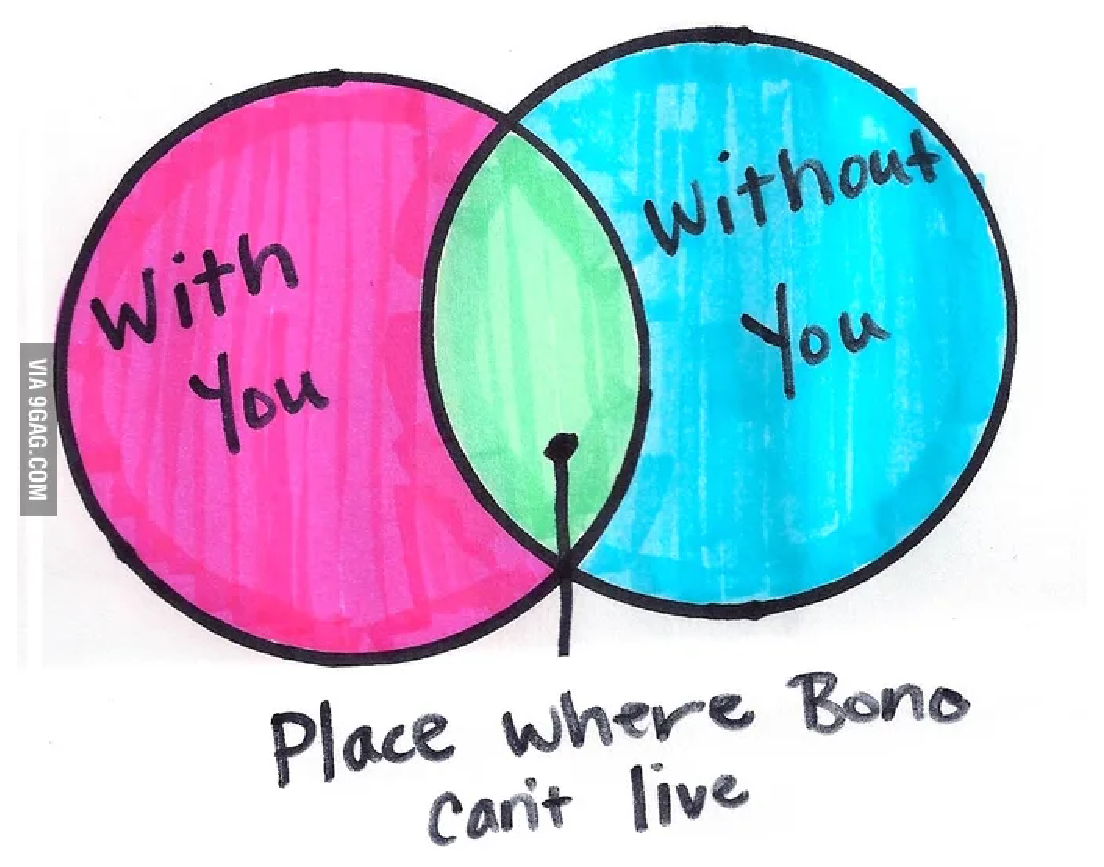
\includegraphics[scale=.3]{fig/bonoVenn.eps}
\end{minipage}

\medskip

\noindent
{\em From Section~\ref{section:setProofs}}

\begin{requ}
Let $A$ and $B$ be sets.
\begin{lenum}
\item
Let's say that I can prove that whenever $x\in A$, then $x\in B$.
What did I just prove?
\item
Let's assume I have the proof from part (a), but I can also prove that 
whenever $x\in B$, then $x\in A$. Now what have I proven?
\end{lenum}
\begin{requanswer}
(a) $A\subseteq B$.
(b) $A=B$.
\end{requanswer}
\end{requ}

\begin{requ}
Give an informal proof of the second version of De Morgan's law (See Table~\ref{table:setIdentities})
by describing the sets on both sides of the inequality and concluding that they are the same.
\begin{requanswer}
First, $A\cap B$ is the set of elements that are in both $A$ and $B$. Therefore, 
$\overline{A\cap B}$  is the set of elements that are not in both $A$ and $B$.
(This includes elements that are in $A$ but not $B$, in $B$ but not $A$, or in neither $A$ nor $B$.)
$\overline{A}\cup\overline{B}$ is the union of the elements that are not in $A$ and the elements that are not in $B$.
That is, it is any element that is either not in $A$ or not in $B$. So it is all elements that are not in both $A$ and $B$,
which is exactly what $\overline{A\cap B}$ is.
Therefore, $\overline{A\cap B}= \overline{A}\cup\overline{B}$.
\end{requanswer}
\end{requ}

\begin{requ}
Use a set containment proof to prove the first complement law. 
That is, if $A$ is a set and $U$ is the universal set, prove that $A\cup \overline{A}=U$.
\begin{requanswer}
First, notice that since $U$ is the universal set, $A\subseteq U$ and $\overline{A}\subseteq U$.
Let $x\in A\cup \overline{A}$. Then either $x\in A$ or $x\in\overline{A}$.
In either case, $x\in U$ (since $A\subseteq U$ and $\overline{A}\subseteq U$). Therefore $A\cup \overline{A}\subseteq U$.

Now, assume $x\in U$.  If $x\in A$, then $x\in A\cup \overline{A}$.
If $x\not\in A$, then by definition, $x\in\overline{A}$, and therefore $x\in A\cup \overline{A}$.
In either case, $x\in A\cup \overline{A}$. Therefore $U\subseteq A\cup \overline{A}$.

Since we proved containment both ways, $A\cup \overline{A}=U$.
\end{requanswer}
\end{requ}

\medskip
\noindent
{\em From Section~\ref{section:moddiv}}

\begin{requ}
How can you use the $\bmod$ operator to determine
whether an integer is even or odd?
\begin{requanswer}
Given an integer $a$, compute $a\bmod 2$.
If it is $0$, $a$ is even, and if it is $1$, $a$ is odd.
\end{requanswer}
\end{requ}


\begin{requ}
If you want to know what time it is 8 hours from now, can you use modular arithmetic to help you compute that?
Explain.
Does the answer change in any way if you are working with 24-hour military time versus 12-hour times with am/pm?
Explain how the calculation can be done in both cases (using modular arithmetic, assuming it is appropriate).
\begin{requanswer}
It certainly can be used. If the current time is $t$, and you are on 24-hour time, 
then in 8 hours the time will be $(t+8 \bmod 24$. If you are using 12-hour time, it is a little more complicated.
You can compute $(t+8)\bmod 12$ to get the time in 8 hours, but if the result is $0$, 
you need to treat it like 12. 
Also, this does not take into account whether there was a switch from am to pm.
That is more complicated and we would need to use additional logic to get that part correct.
\end{requanswer}
\end{requ}

\begin{requ}
Given integers $a$, $b$, and $n$, 
explain how you can determine whether or not 
$a\equiv b\pmod n$. Hint: There may be a helpful Theorem
from this section.
\begin{requanswer}
Compute $c=a\bmod n$ and $d=b\bmod n$.
According to Theorem~\ref{thm:congruence}, 
$c=d$ if and only if $a\equiv b\pmod n$. 
so just determine whether or not $c=d$.
\end{requanswer}
\end{requ}


\begin{requ}
Compute $\gcd(67890,12345)$ using Euclid's algorithm.
\begin{requanswer}
$\gcd(524,118)=15$ as demonstrated here: 

\begin{tabular}{|l|l|l|l|}
\hline
step&a&b&r\\
\hline
\hline
1&67890&12345&6165\\
\hline
2&12345&6165&15\\
\hline
3&6165&15&0\\
\hline
4&15&0&0\\
\hline
\end{tabular}
\end{requanswer}
\end{requ}

\begin{requ}
Are 67890 and 12345 relatively prime? Explain.
\begin{requanswer}
They are not because they have a common factor of 15.
\end{requanswer}
\end{requ}


\begin{requ}
Is the floor of the ceiling of a number always the same as the ceiling of the floor of a number? 
Explain, giving examples as necessary.
\begin{requanswer}
No. In fact, they are usually not going to be the same (unless you start with an integer).
As an example, the floor of 3.2 is 3, and the ceiling of 3 is 3, so the ceiling of the floor of 3.2 is 3. 
The ceiling of 3.2 is 4, and the floor of 4 is 4, so the floor of the ceiling of 3.2 is 4.
\end{requanswer}
\end{requ}


\medskip
\noindent
{\em From Section~\ref{section:functionDefs}}



\begin{requ}
Let $f:\BBZ \rightarrow \BBZ$ be a function defined by $f(x)=2x$.
\begin{lenum}
\item What is the domain of $f$? 
\item What is the codomain of $f$? 
\item What is the range of $f$? 
\end{lenum}
\begin{requanswer}
(a) $\BBZ$. (b) $\BBZ$. (c) $\{2z | z\in\BBZ\}$. That is, the set of all even numbers.
\end{requanswer}
\end{requ}

\begin{requ}
Let $A=\{1,2,3,4\}$ and $B=\{2,4,6,8\}$.
Give an example of each of the following. If it is not possible, explain why.
\begin{lenum}
\item A function $f:A\rightarrow B$ that is one-to-one.
\item A function $f:A\rightarrow B$ that is not one-to-one.
\item A function $f:A\rightarrow B$ that is onto.
\item A function $f:A\rightarrow B$ that is not onto.
\item A function $f:A\rightarrow B$ that is bijective.
\end{lenum}
\begin{requanswer}
Here are possible answers. There are many other possible correct answers.
(a) $f(x)=2x$.
(b) $f(x)=6$.
(c) $f(x)=2x$.
(d) $f(x)=4$.
(e) $f(x)=2x$.
\end{requanswer}
\end{requ}

\begin{requ}
Let $A=\{1,2,3,4\}$ and $B=\{2,4,6,8,10,12\}$.
Give an example of each of the following. If it is not possible, explain why.
%and/or fix the flaw in the statement (if there is an easy fix). % I'm not sure what I meant by this. CAC, 6/9/2020
\begin{lenum}
\item A function $f:A\rightarrow B$ that is one-to-one.
\item A function $f:A\rightarrow B$ that is not one-to-one.
\item A function $f:A\rightarrow B$ that is onto.
\item A function $f:A\rightarrow B$ that is not onto.
\item A function $f:A\rightarrow B$ that is bijective.
\end{lenum}
\begin{requanswer}
Here are possible answers. There are many other possible correct answers.
(a) $f(x)=2x$.
(b) $f(x)=(2x)\bmod 6$ (so $f(4)=2$ instead of 8).
(c) Impossible. The domain only has 4 numbers, and the codomain has 6, so it is impossible to map to all of them.
(d) $f(x)=2x$ (it doesn't map to 10 or 12).
(e) Impossible. Since an onto function is impossible, a bijective one is as well.
\end{requanswer}
\end{requ}

\begin{requ}
Let $f(x)=2^x$ and $g(x)=x+2$. Find $f\circ g$ and $g\circ f$.
\begin{requanswer}
$(f\circ g)(x)=2^{x+2}$ and $(g\circ f)(x)=2^x+2$.
Did you get them backwards? If so, look at the definition of composition of functions again.
\end{requanswer}
\end{requ}

\medskip
\noindent
{\em From Section~\ref{section:functionProofs}}

\begin{requ}
Is each of the following true or false? If it is false, explain why.
\begin{lenum}
\item To show that $f$ is one-to-one, you need to show that if $a=b$, then $f(a)=f(b)$.
\item To show that $f$ is {\em not} one-to-one, you only need to find two values in the domain that map
to the same element of the codomain.
\item To show that $f$ is onto, you need to show that every element of the domain gets mapped to some element
of the codomain.
\item To show that $f$ is onto, you can show that the range and codomain are exactly the same set.
\item To show that $f$ is {\em not} onto, you need to show that no elements of the range are mapped to.
\item To show that $f$ is invertible, you need to show that $f$ is one-to-one and that $f$ is onto.
\end{lenum}
\begin{requanswer}
(a) False. If $a=b$, then clearly $f(a)=f(b)$, so that's meaningless. You need to show that if $f(a)=f(b)$, then $a=b$. 
(b) True.
(c) False. That's the definition of a function. to show onto, you need to show that every element of the codomain 
gets mapped to by some element of the domain.
(d) True. Since the range is the set of values actually mapped to, if it equals the codomain, then every value is mapped
to and the function is onto.
(e) False. For two reasons. First, elements of the range are always mapped to--that's the definition of range.
Even if you change range to codomain, it is still false. You only need to show that there is at least one element of the
codomain that is not mapped to.
(f)True.
\end{requanswer}
\end{requ}


\begin{requ}
Let $f:\reals\rightarrow\reals$ be defined by
$f(x)=x^3-8$. Prove that $f$ is invertible and find its inverse.
\begin{requanswer}
First, notice that if $f(a)=f(b)$, then $a^3-8=b^3-8$,
which implies $a^3=b^3$. Taking the third root of each side,
we get $a=b$. Thus, $f$ is one-to-one.
Now, notice that if $x\in\reals$, then $\sqrt[3]{x+8}\in \reals$,
and $f\left(\sqrt[3]{x+8}\right)=\left(\sqrt[3]{x+8}\right)^3-8=x+8-8=x$,
so $f$ is onto.
To find the inverse (which I already did in order to prove it was
onto, but I'll show the work anyway), 
we solve $y=x^3-8$ for $x$. We get $x^3=y+8$, so
$x=\sqrt[3]{y+8}$. Replacing variables, we have
that $f^{-1}=\sqrt[3]{x+8}$.
\end{requanswer}
\end{requ}

\medskip
\noindent
{\em From Section~\ref{section:parts}}

\begin{requ}
Let $A=\{1,2,3,4,5,6,7,8,9,10\}$, $B=\{2,4,6,8,10\}$.
\begin{lenum}
\item Define a set $C$ such that $B, C$ is a partition of $A$. 
\item Define a set $C$ such that $B, C$ is a not partition of $A$ because the sets are not disjoint. 
\item Define a set $C$ such that $B, C$ is a not partition of $A$ because the union of the sets is not $A$.
\item Define sets $C$ and $D$ such that $B, C, D$ is a partition of $A$. 
\item Define sets $C$ and $D$ such that $B\cap D=C\cap D=\emptyset$, 
and $B\cup C\cup D=A$, but $B, C, D$,  is a not partition of $A$. 
\end{lenum}
\begin{requanswer}
(a) $C=\{1,3,5,7,9\}$.
(b) $C=\{1,2,3,5,7,9\}$ (or any set that contains all of 1,3,5,7,9, and at least one of 2, 4, 6, 8, or 10).
(c) $C=\{1,3,7,9\}$ (or any proper subset of $\{1,3,5,7,9\}$).
(d) $C=\{1,3,5\}$ and $D=\{7,9\}$ (or any two disjoint sets such that $C\cup D=\{1,3,5,7,9\}$.
(e) $C=\{1,2,3,5\}$ and $D=\{7,9\}$ (or many other possibilities).
\end{requanswer}
\end{requ}

\begin{requ}
Is $\{(1,3), (456, 901), (867,5309)\}$ a relation on $\BBZ$? Explain.
\begin{requanswer}
Yes. It is a subset of $\BBZ\times\BBZ$.
\end{requanswer}
\end{requ}


\begin{requ}
Define a partial order on the set of all human beings. Briefly explain why it is a partial order.
\begin{requanswer}
There are many possible answers. Here is one.
Define $T$ to be the relation on human beings such that $x T y$ if and only if $x$ is at least as tall as $y$.
It is not hard to see that $T$ is reflexive, anti-symmetric, and transitive, so it is a partial order.
\end{requanswer}
\end{requ}

\begin{requ}
Define an equivalence relation on the set of all cars. 
Briefly explain why it is an equivalence relation.
Then define a partition of the set of all cars that corresponds to the equivalence relation.
Give a clear definition of each equivalence class (that is, each set in the partition), 
and if possible give a representative element from each subset.
\begin{requanswer}
answers we vary, but here is one possibility.
Let $C$ be the set of all cars.
Define the relation $R$ on $C$ by $x R y$ if and only if $x$ was manufactured in the same year as $y$.
It is not hard to see that $R$ is symmetric, reflexive, and transitive, so it is an equivalence relation.
Let $C_y$ be the set of all cars manufactured in year $y$.
Then it is not hard to see that $C=C_{1886}\cup C_{1887}\cup\cdots\cup C_{2023}\cup C_{2024}\cup C_{2025}$
is a partition of $C$ (assuming you aren't reading this in 2026 or later, and assuming we regard 1886 as the first year
a car was made, which turns out to be a question without a clear answer).
For a representative for class $C_y$, simply pick any car that was manufactured in year $y$.
\end{requanswer}
\end{requ}

\begin{requ}
Let $B$ be the relation on $\BBZ^+$ such that $(x,y)\in B$ if $x$ and $y$ have the same number of
1s in their binary representation. For example, $3=11_2$ and $5=101_2$, 
so both $3$ and $5$ have two 1s in their binary representation. 
Thus,  $(3,5)\in B$ and $(5,3)\in B$. 
On the other hand, $(3,2)\not\in B$ since
$2=10_2$ has only one 1 in its binary representation.
\begin{lenum}
\item Is $B$ an equivalence relation? Explain.
\item Is $B$ a partial order? Explain.
\item Define a partition of $\BBZ^+$ based on the relation $B$.
(Hint: The fact that I am asking this question should clue you in on the answer to one or more 
of the previous questions.) 
In other words, define sets 
$B_1, B_2, B_3\ldots$ such that $\BBZ^+ = B_1\cup B_2\cup B_3\cup\cdots$
and $B_i\cap B_j=\emptyset$ if $i\not = j$.
To be clear, I am looking for a clear definition of $B_i$ for a given value of $i$.
\item
Give the most obvious choice of a representative for each subset $B_i$.
That is, choose an $a_i$ such that $[a_i]=B_i$.
\item 
Give at least 4 elements of $B_2$.
\end{lenum}
\begin{requanswer}
(a) It is straightforward to prove that $B$ is symmetric, reflexive, and transitive, so it is an equivalence relation.
(b) It is not. It is no anti-symmetric.
(c) Let $B_i$ be the positive integers that have $i$ ones in their binary representation.
It is easy to see that $B_i\cap B_j=\emptyset$ if $i\not = j$ and that  $\BBZ^+ = B_1\cup B_2\cup B_3\cup\cdots$,
so this definition gives us a partition of $\BBZ^+$.
(d) We just let $a_i$ be the number whose binary representation is $i$ 1s.
For instance, $a_1=1$, $a_2=3$, $a_3=7$, etc. Notice that we can do better by defining it explicitly: $a_i=2^i-1$.
(e) The smallest elements of $B_2$ would be $3=11_2$, $5=101_2$, $6=110_2$, and $9=1001_2$. 
There are infinitely many other possible answers.
\end{requanswer}
\end{requ}
